\section{Results}
\subsection{Survey results in summary}
\justify

%- Present results in the order of the research questions
%- (Amount of records, amount of faulty records)
%- Uncertainties
%- Present logically all results and interesting specific questions
%- Compare parking with original Travel Time Matrix values and values collected by me
%- Charts, statistics
%- Just show your findings, no nonsense
In this chapter, the thesis research survey results which fit the criteria as per shown in \hyperref[sec:processdata]{\fullref{sec:processdata}} is discussed. Within the selected criteria (\code{parktime < 60} and \code{walktime < 60}), the survey received a total of 5579 visits from 4320 unique IP addresses. 848 unique IP addresses visited the survey more than one time and in total 1060 unique IP addresses sent data to the survey. 24.5 percent of all visitors submitted at least one data row. On average one respondent submitted 4.9 data rows.

The survey received in total 5183 data rows. All postal code areas were represented in the survey results (figure~\ref{fig:postalvis_answers}), but the data row count histogram was heavily skewed to the right, with the first quartile being eight data rows, second (median) 17 data rows and third 42 data rows (table~\ref{tab:muns_answer_stats}, figures~\ref{fig:parktime_hist},~\ref{fig:walktime_hist}). Most respondents reported short parking times below ten minutes, but the histograms do not smoothly lessen in values from the right to left, as people have preferred to report round figures such as five, ten, or fifteen minutes. There were five postal code areas with more than one hundred data rows and 55 postal code areas with less than ten data rows. In Helsinki, the answers strongly clustered around the center of Helsinki, with other centers of activity being Herttoniemi and Itäkeskus-Marjaniemi in Helsinki, Tapiola-Otaniemi and Leppävaara in Espoo, and Tikkurila-Vantaanportti in Vantaa.

\begin{figure}[H]%
    \centering
    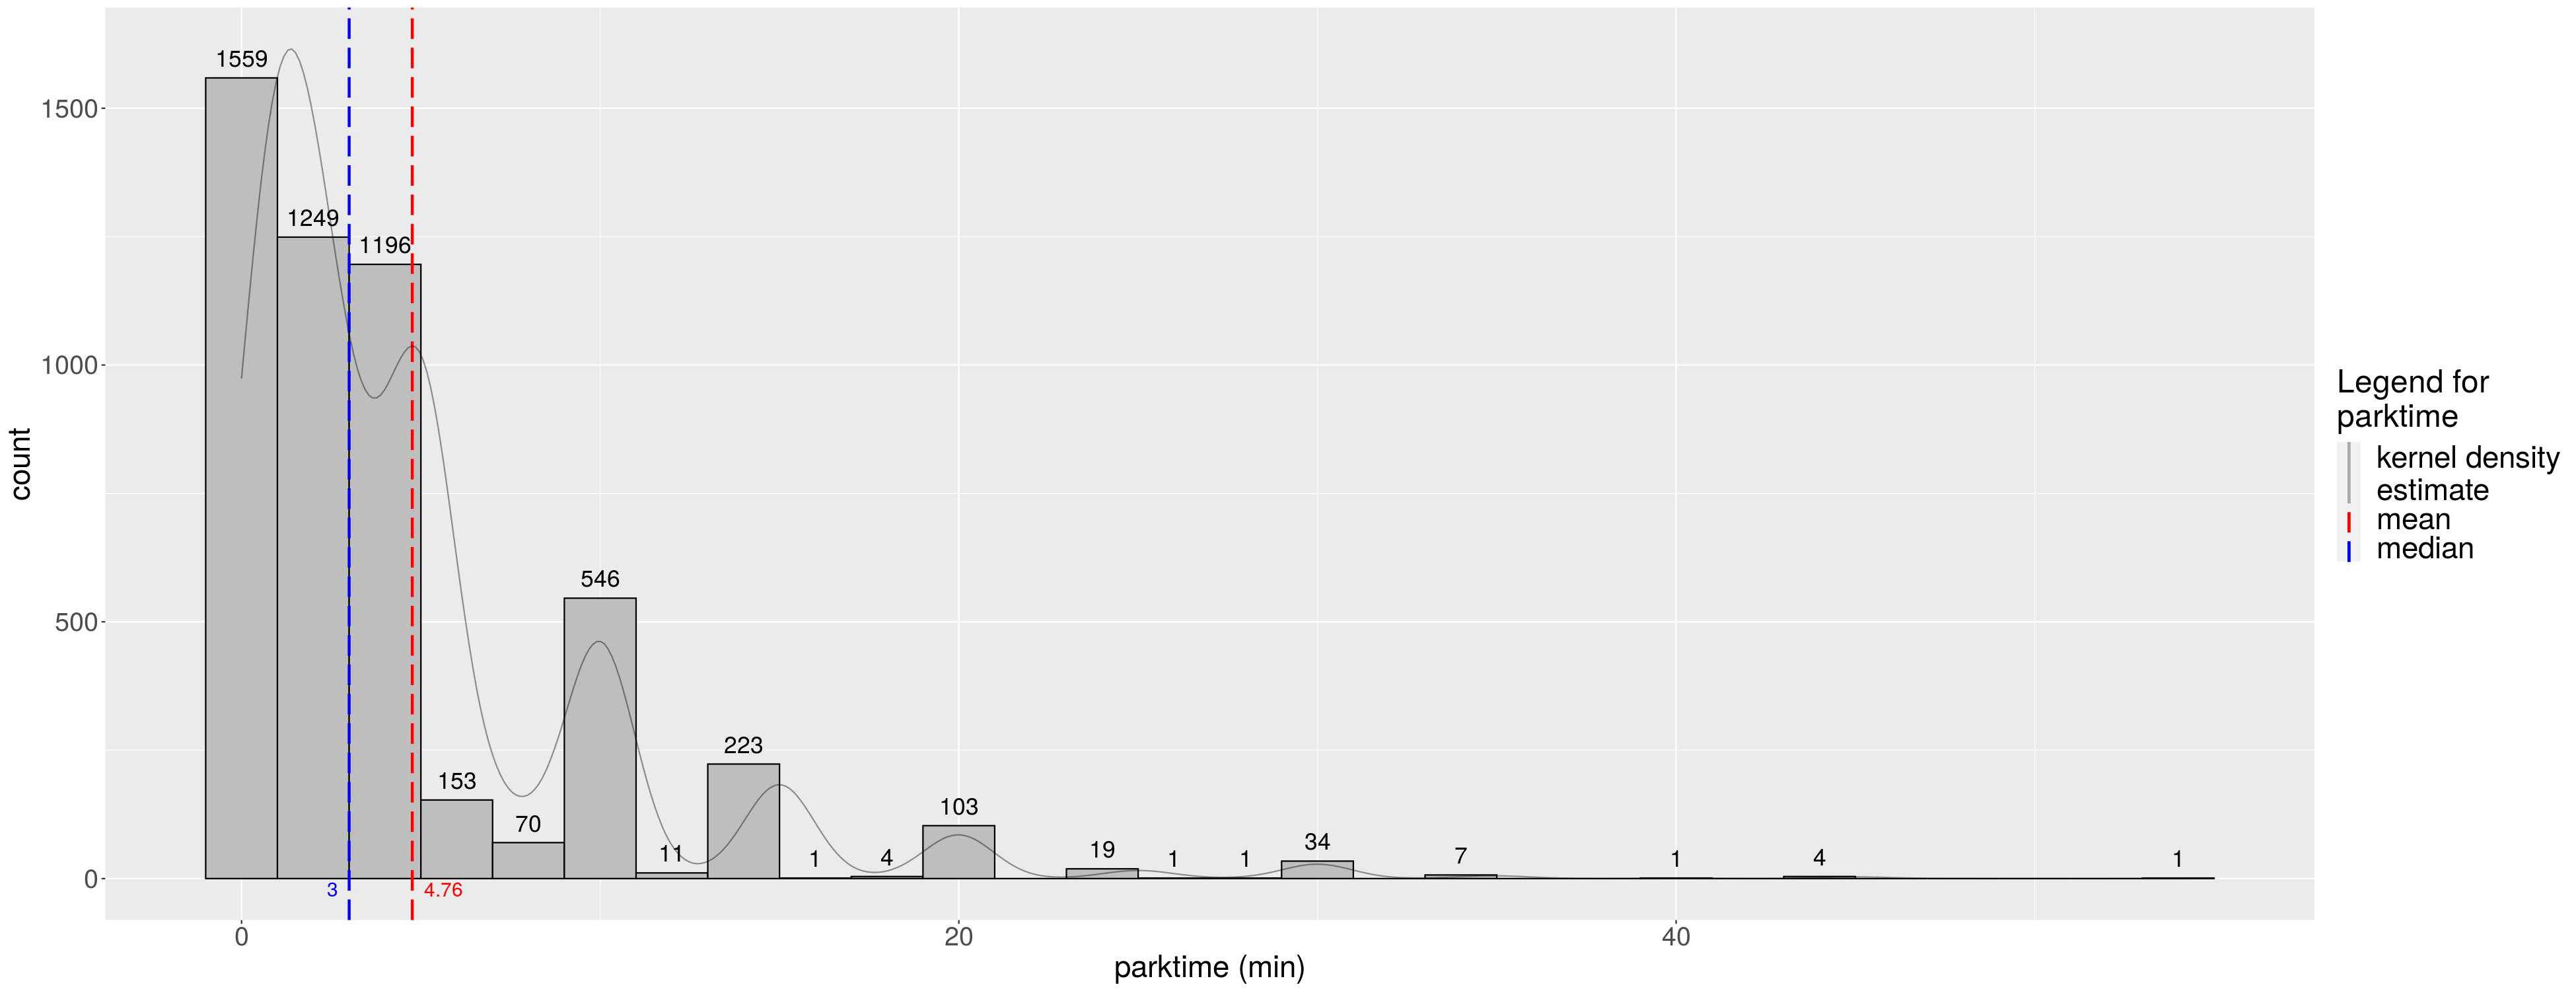
\includegraphics[width=\textwidth]{images/hist_pmax59-wmax59_parktime-likert_binw2_02-08-2020.png}
    \caption[Histogram, searching for parking]{All permitted thesis survey \code{parktime} values (< 60) shown on histogram.}%
    \label{fig:parktime_hist}%
\end{figure}

\begin{figure}[H]%
    \centering
    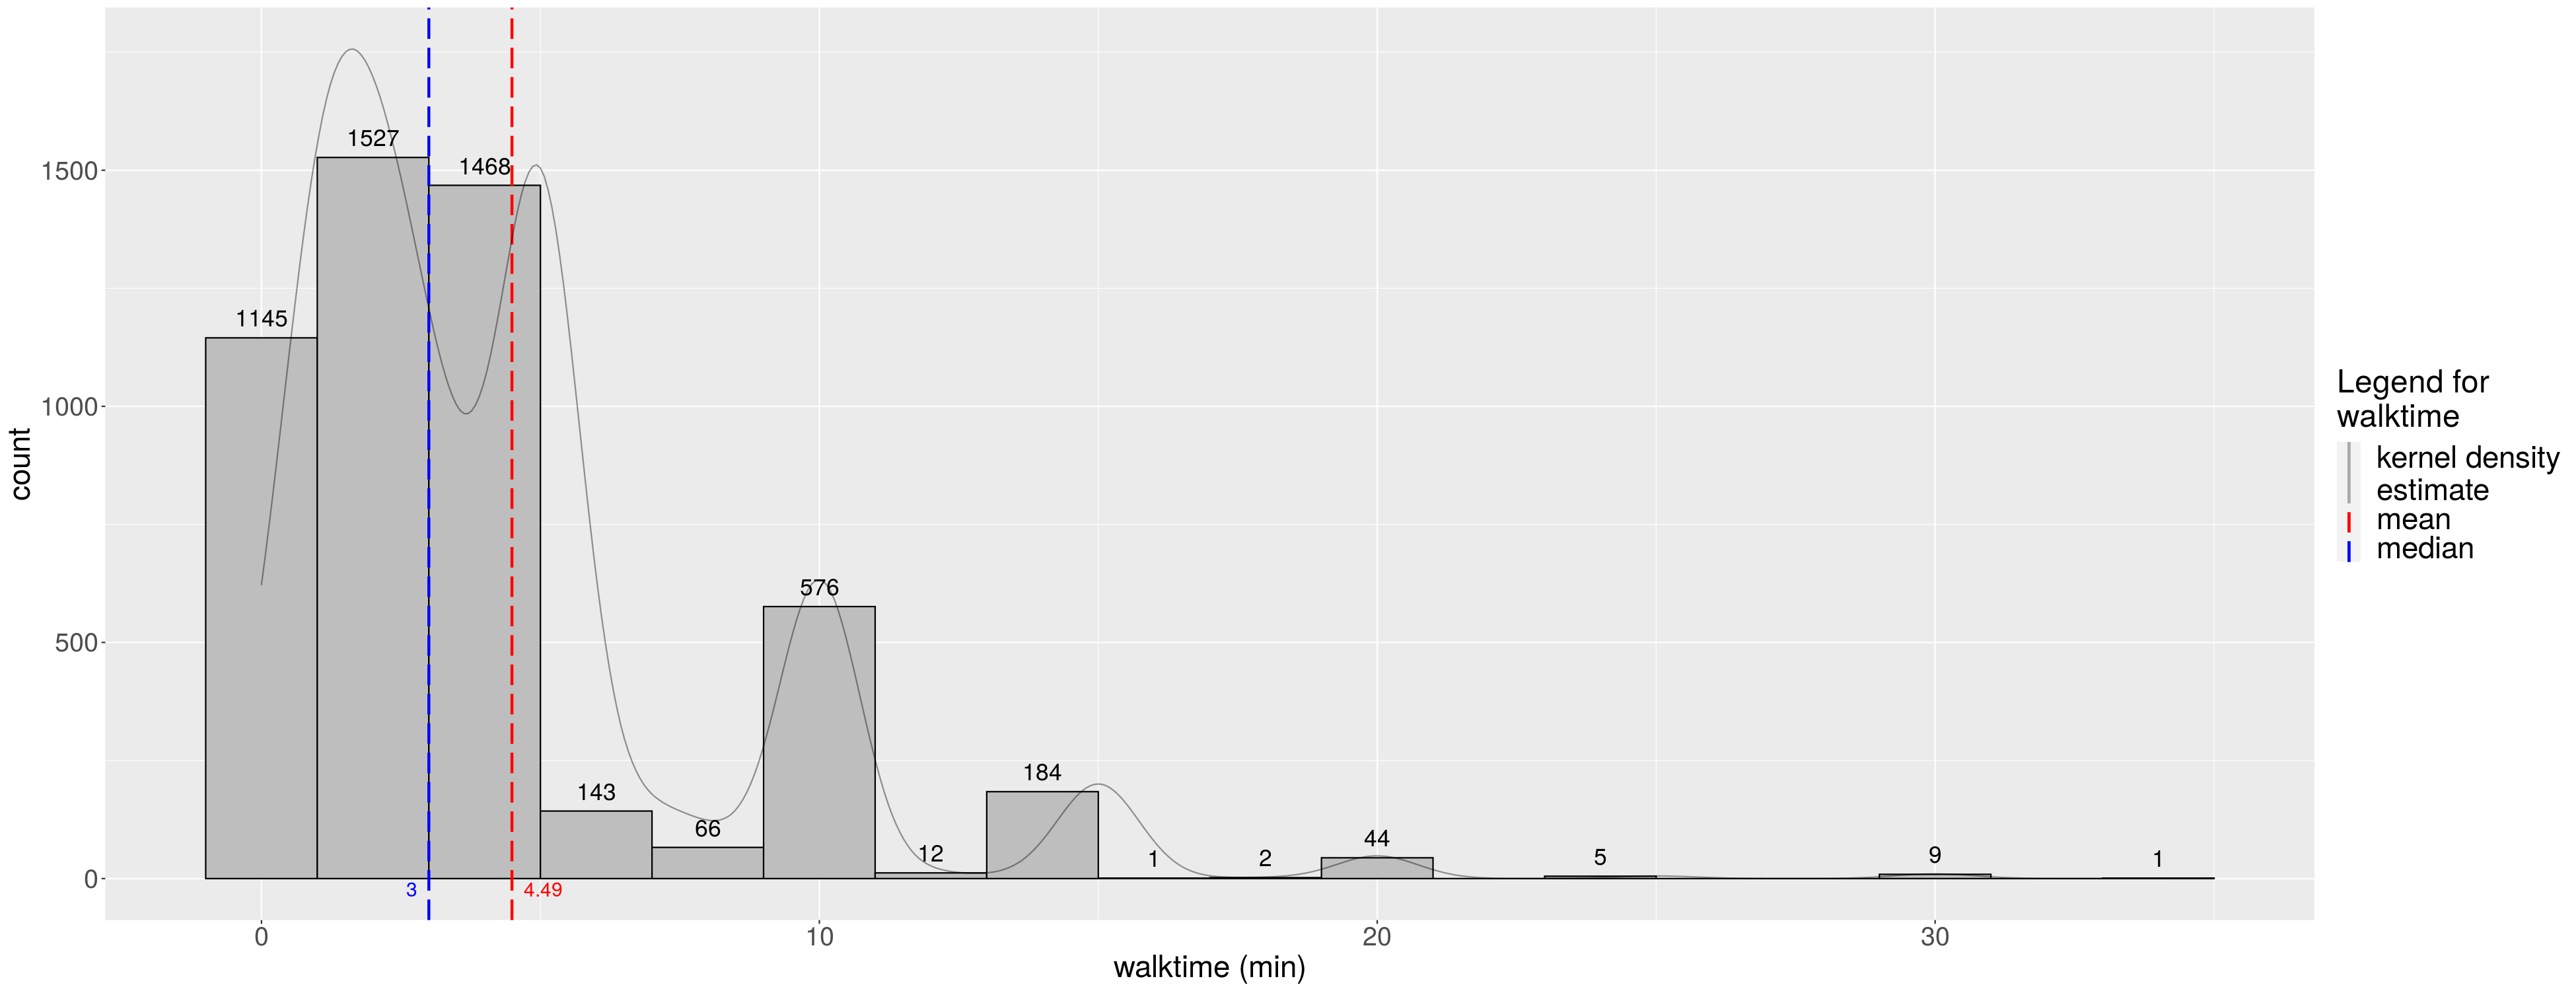
\includegraphics[width=\textwidth]{images/hist_pmax59-wmax59_walktime-likert_binw2_02-08-2020.png}
    \caption[Histogram, walk to destination]{All permitted thesis survey \code{walktime} values (< 60) shown on histogram.}%
    \label{fig:walktime_hist}%
\end{figure}

\begin{hyphenrules}{nohyphenation}
    \begin{table}[H]
        \centering
        \def\arraystretch{1.2}
        \setlength\tabcolsep{4pt}
        \caption[Answer counts by municipality]{Amount of data rows received per municipality in Helsinki Capital Region.} 
        \label{tab:muns_answer_stats}
        \begin{tabular}{ @{} >{\raggedright\arraybackslash}p{3cm} >{\raggedright\arraybackslash}p{2cm} >{\raggedright\arraybackslash}p{4cm} >{\raggedright\arraybackslash}p{2cm} >{\raggedright\arraybackslash}p{2cm} @{} }
            \toprule
            Municipality & Data rows total & Most data rows in municipality & Data rows mean in municipality & Data rows median in municipality \\
            \midrule
            Helsinki & 3777 & 271 (00100 Helsinki Keskusta - Etu-Töölö) & 45.0 & 34.5 \\
            Espoo & 637 & 84 (02600 Etelä-Leppävaara) & 17.7 & 9 \\
            Vantaa & 746 & 91 (01510 Kirkonkylä-Veromäki) & 16.2 & 8 \\
            Kauniainen & 23 & 23 (02700 Kauniainen) & 23 & 23 \\
            % use \usepackage[table]{xcolor} and \usepackage{booktabs} to define \greyrule
            \greyrule
            All & 5183 & 271 (00100 Helsinki Keskusta - Etu-Töölö) & 31.0 & 17 \\
            \bottomrule
        \end{tabular}
    \end{table} 
\end{hyphenrules}

On a closer look to the municipalities, finer details become apparent (figure~\ref{fig:postalvis_answers}). For example, in Helsinki, a wedge-like area of survey activity in the direction of southwest-northeast is visible. Starting out from the west, this area spans from Lauttasaari to the center of Helsinki and moving on all the way east to Malmi. Many of the areas which could be roughly characterised as residential areas were left with little activity. Furthermore, in the survey instructions respondents were requested to refrain from including parking activity in private property, as it was assumed in survey design phase that these areas would provide near to instantaneous parking, potentially distorting the data and obfuscating the objectives set by the thesis research questions. The lightness of activity in residential areas corresponds with the made request.

% A known issue with these maps: Vartiosaari is represented on these maps. As an unreachable island, it shouldn't.
\begin{figure}[H]%
    \centering
    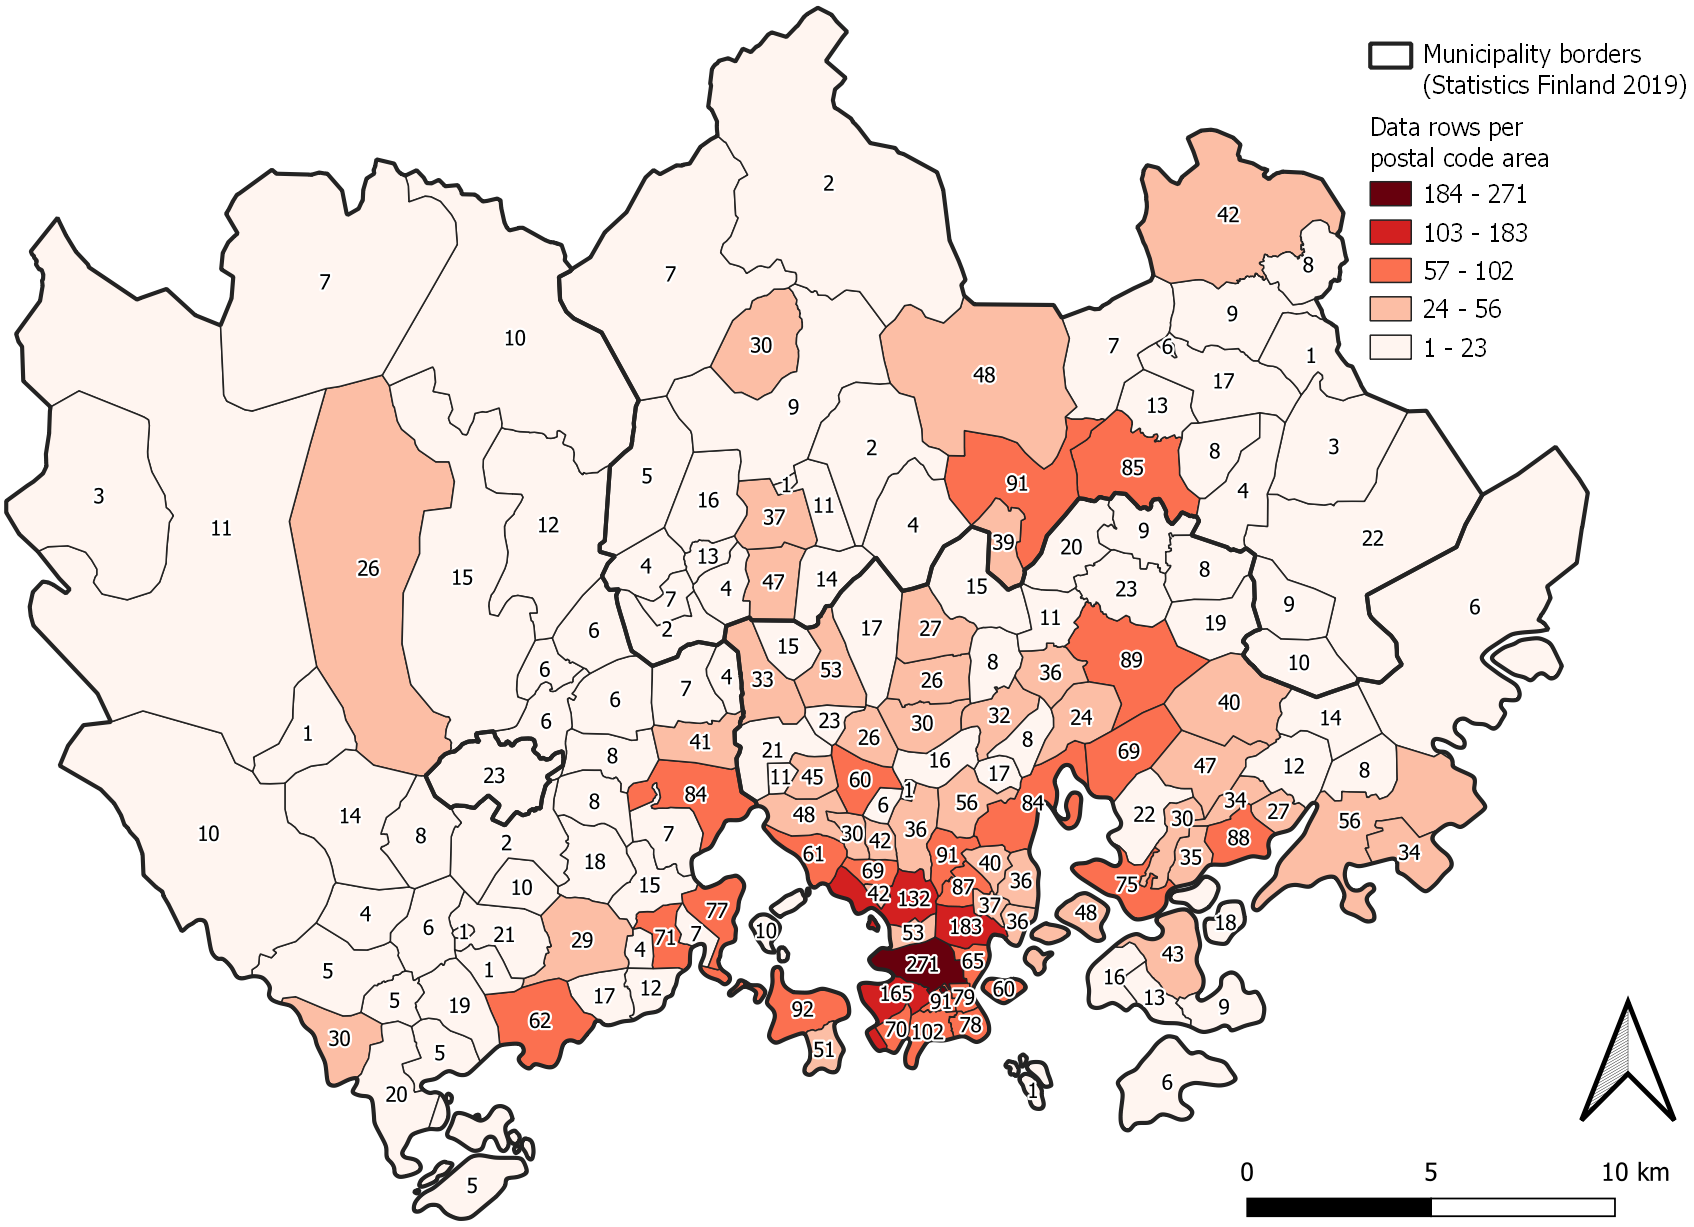
\includegraphics[width=\textwidth]{images/thesis_postalvis_answers.png}
    \caption[Data rows received per postal code area]{This figure illustrates the responses received in the thesis survey per postal code area (n=167). Classes are in natural breaks (Jenks). Municipality borders are based on \textit{postal} data. There are slight differences to the actual municipality boundaries.}%
    \label{fig:postalvis_answers}%
\end{figure}

In the finest resolution available, the postal code areas, long \code{parktime} values closely follow areas with most survey activity (table~\ref{fig:postalvis_parkmean}, table~\ref{fig:postalvis_parkmedian}). The longest \code{parktime} values were encountered in the center of Helsinki, where the mean value for 00120 Punavuori was 10.6 minutes (median 10.0 minutes, 91 data rows) and 00290 Meilahden sairaala-alue 9.4 minutes (5.0 min, 42 data rows). Long parking times over five minutes were recorded in all over the center area, but also in 00570 Kulosaari (mean 5.3 minutes, median 5.0 minutes, 48 data rows) and 00590 Kaitalahti (6.5 min, 3.5 min, 16 data rows). In Espoo, the longest \code{parktime} values were found in 02230 Matinkylä (5.1 min, 5.0 min, 62 data rows), 02100 Tapiola (4.6 min, 3.0 min, 71 data rows), and in 02320 Espoonlahti (4.3 min, 3.0 min, 30 data rows). In Vantaa, it took the longest to find a parking spot in 01300 Tikkurila with (6.4 min, 5.0 min, 85 data rows). According to the survey results, it was relatively hard to find a parking spot in 01700 Kivistö (5.7 min, 4.0 min, 30 data rows), too.

In the case of this survey dataset it is important to not lose sight of median, as mean is susceptible to outliers, of which there are many present. One such situation may be viewed in 01750 Keimola, where the mean \code{parktime} is 5.9 minutes, and median reads at 1.0 minute. In Keimola's situation, one respondent entered a \code{parktime} value of 25 minutes, severely skewing the total sample of seven values. It may be argued that when detecting areas of long duration of searching for parking, median is the better measure to identify areas of interest.

The mean \code{walktime} values follow the same municipal order as those of \code{parktime}: On average, in Helsinki it took 4.8 minutes to walk from one's parked car to the final destination of the journey (table~\ref{fig:postalvis_walkmean}, table~\ref{fig:postalvis_walkmedian}). In Vantaa, this process was 4.0 minutes, while Espoo had mean parking time of 3.9 minutes and Kauniainen 2.2 minutes. Viewing median values, this is 4.0, 3.0, 2.0, and 2.0 minutes for Helsinki, Vantaa, Espoo, and Kauniainen, respectively. Of the entire research area, Espoo's 02780 Kauklahti stood out with a mean walking time of 6.3 minutes (median 5.5 min) to one's destination. It is notable that this subdivision received 10 answers, ranking second to the last before Helsinki's 00890 Östersundom's total of 6 answers.

When viewed through postal code areas, \code{walktime} shows the longest durations to walk from one's car to the final destination in Helsinki with the top belonging to 00100 Helsinki Keskusta -- Etu-Töölö (mean 7.4 minutes, median 5.0 minutes, 271 data rows). Most of the central Helsinki did not fall far behind with most values ranging from five to seven minutes. Outside of the center of Helsinki, 00570 Kulosaari (6.7 min, 5.0 min, 48 data rows), 00590 Kaitalahti (6.3 min, 5.0 min, 16 data rows) and 00690 Tuomarinkylä-Torpparinmäki (5.3 min, 3.0 min, 15 data rows) saw long \code{walktime} values within the boundaries of Helsinki. Looking outward from the capital, the \code{walktime} values in Espoo were mostly lower than those in Helsinki. Longest recorded durations in Espoo were in 02100 Tapiola (5.4 min, 5.0 min, 71 data rows), 02780 Kauklahti (6.3 min, 5.5 min, 10 data rows), and 02820 Nupuri-Nuuksio (7.0 min, 5.0 min, 7 data rows). Vantaa's longest \code{walktime} values were found in 01530 Veromiehenkylä (8.0 min, 5.5 min, 48 data rows), 01300 Tikkurila (6.3 min, 5.0 min, 85 data rows), and 01700 Kivistö (5.6 min, 5.0 min, 30 data rows). 

It is difficult to try and determine the causes behind these long \code{walktime} values, but it may be worth noting, that many of the postal code areas with top values contain popular sightseeing locations, such as the Haltiala domestic animal farm in 00690 Tuomarinkylä-Torpparinmäki and the national park of Nuuksio in 02820 Nupuri-Nuuksio. The postal code area of 01530 Veromiehenkylä is almost entirely in the use of Helsinki-Vantaa Airport. It quickly becomes apparent that recreational trips to Nuuksio National Park may nudge the Espoo's \code{walktime} values upward, while in Vantaa, the Helsinki-Vantaa Airport walking seems to be a similar factor. A summarising feature about \code{walktime} is that areas of long walking times from one's car to the final destination are not as apparently clustered as those of \code{parktime} are.


\begin{figure}[H]%
    \centering
    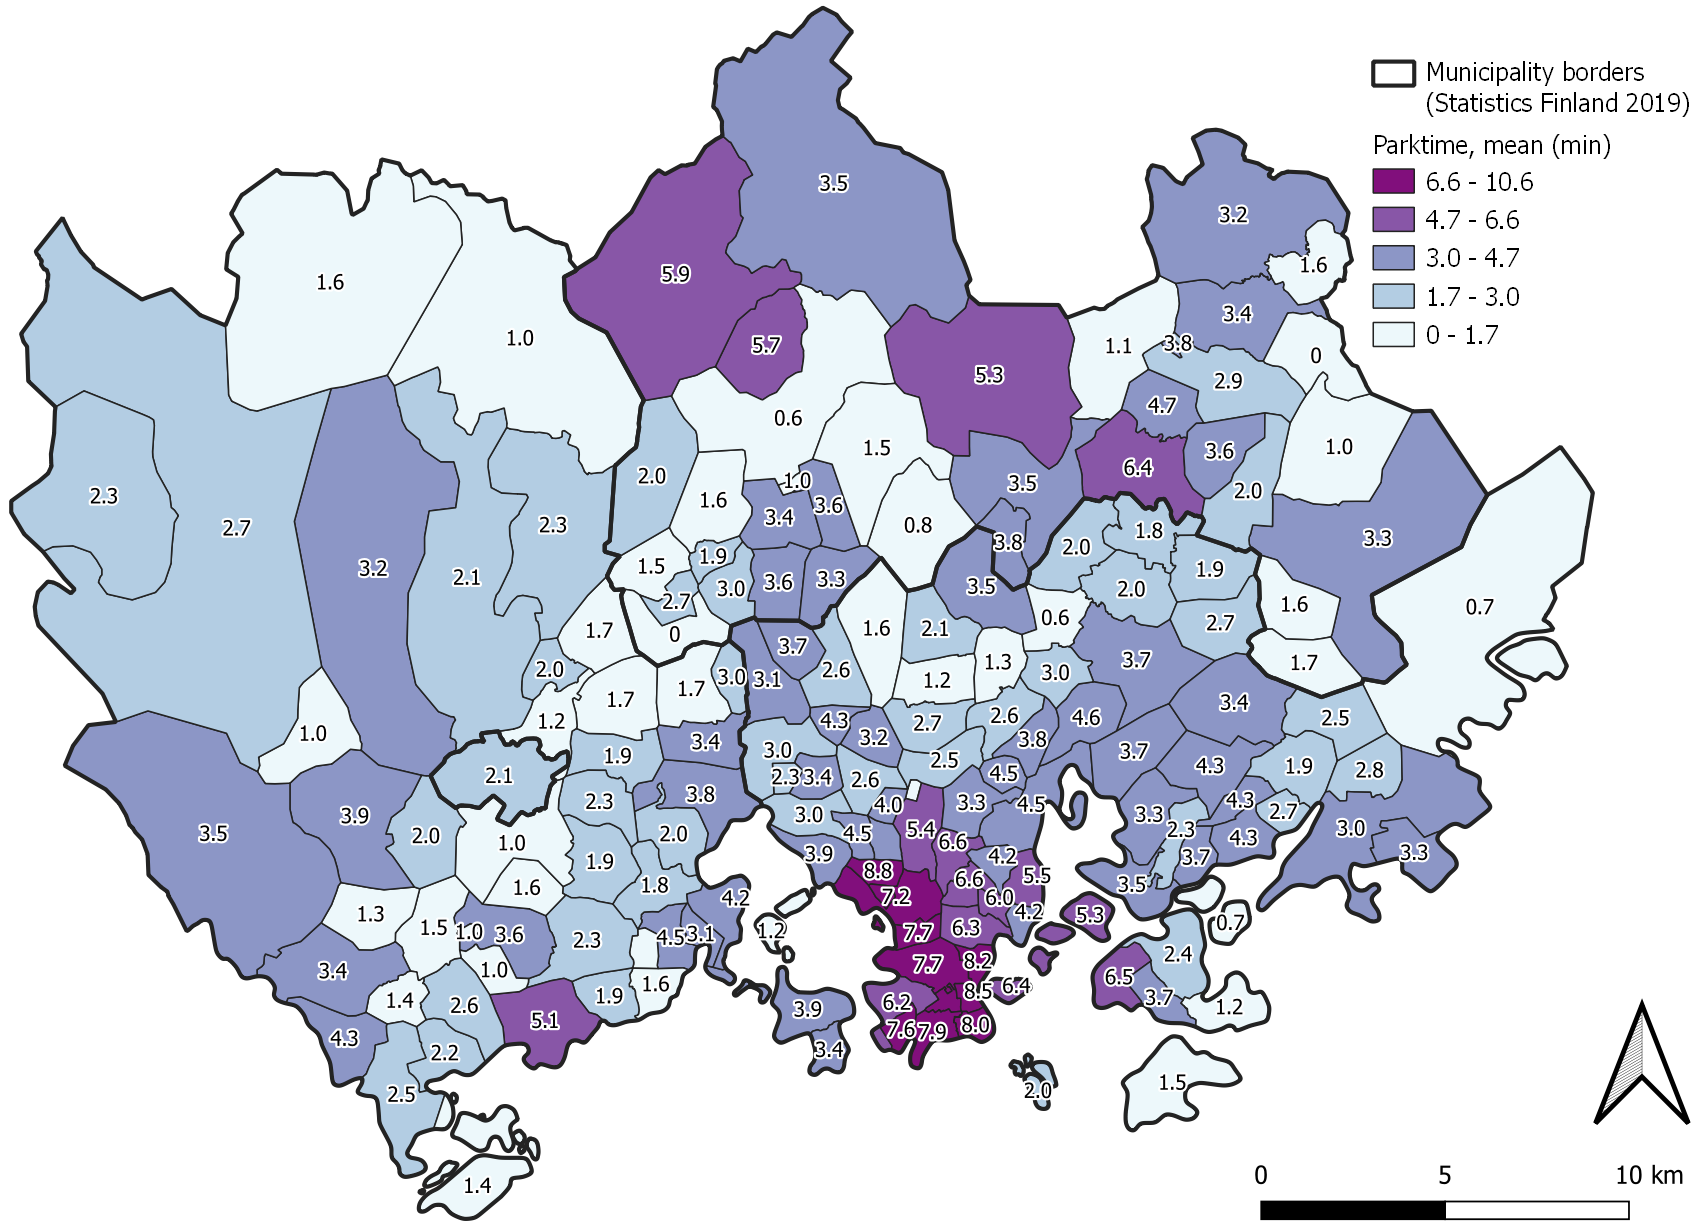
\includegraphics[width=.88\textwidth]{images/thesis_postalvis_parkmean.png}
    \caption[Parktime, mean, in the reseach area]{This figure illustrates the mean duration of searching for parking and parking one's car in each postal code area.}%
    \label{fig:postalvis_parkmean}%
\end{figure}

\begin{figure}[H]%
    \centering
    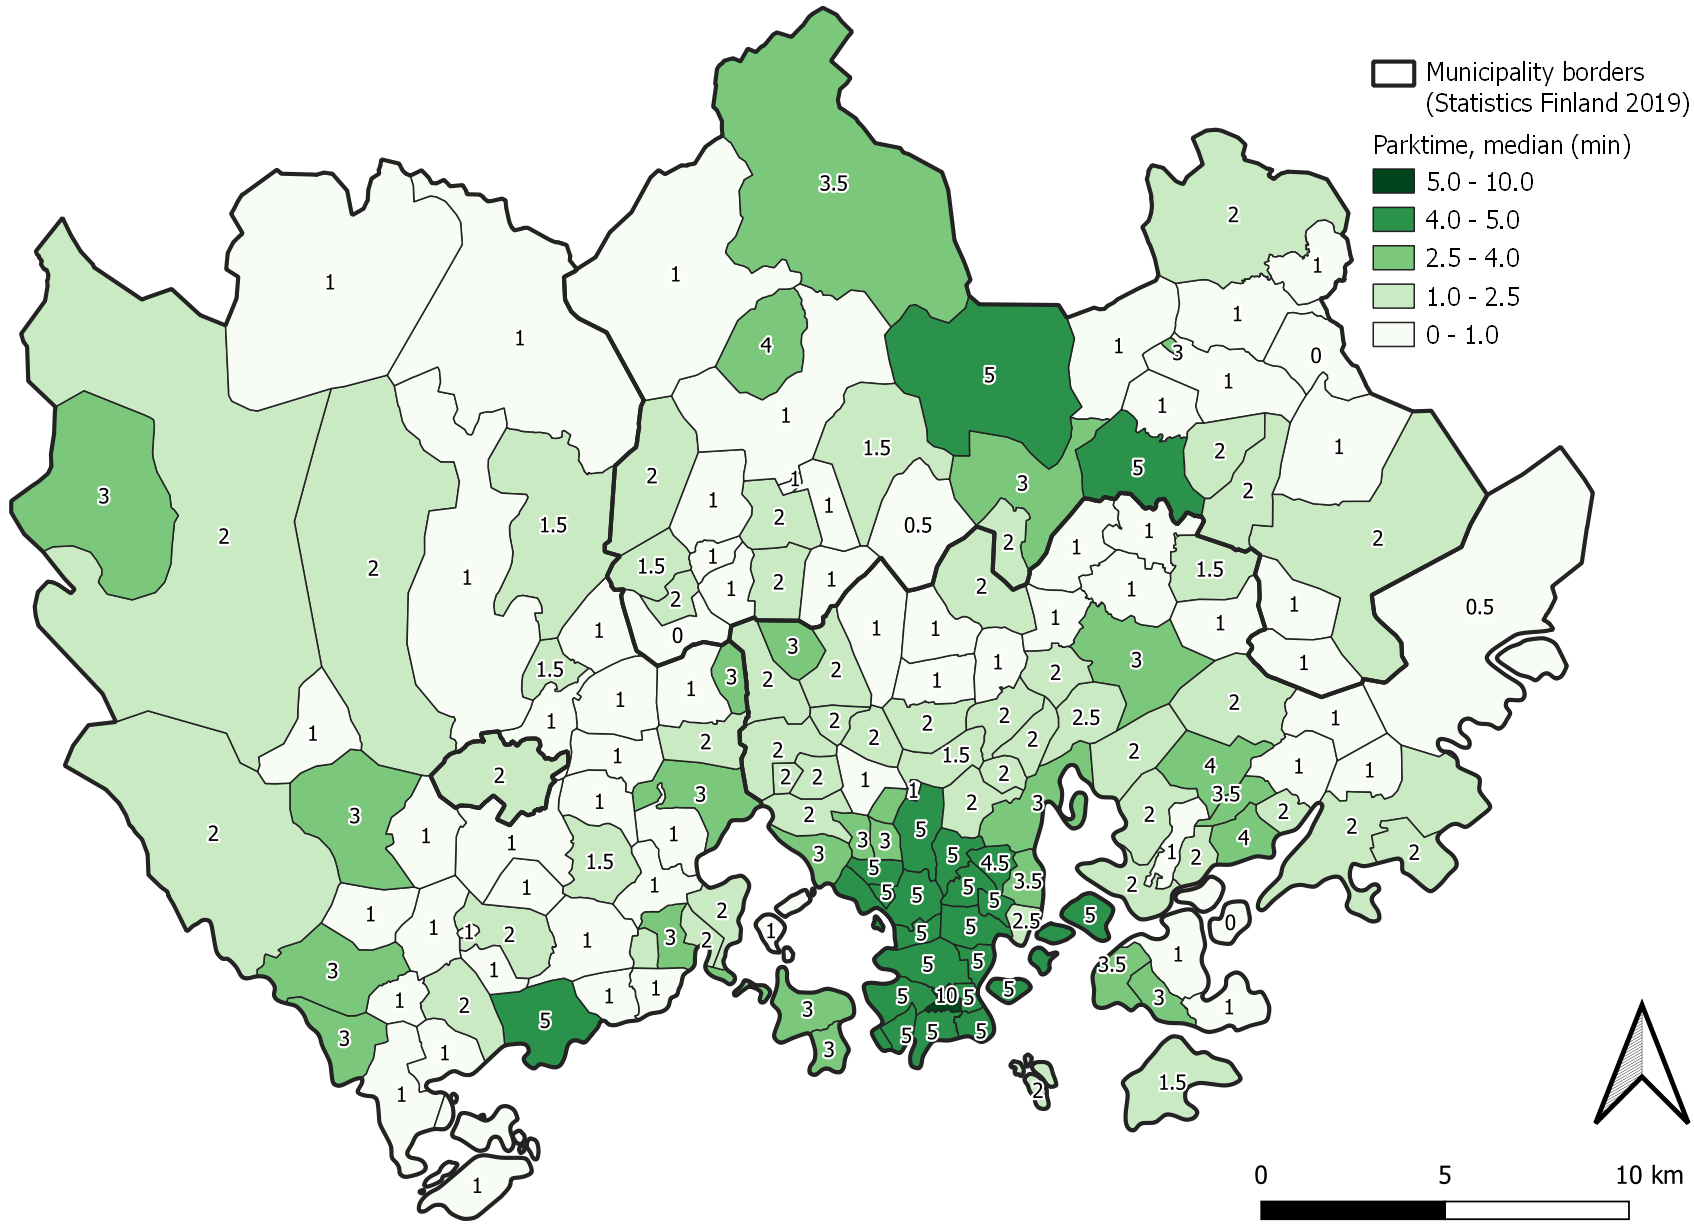
\includegraphics[width=.88\textwidth]{images/thesis_postalvis_parkmedian.png}
    \caption[Parktime, median, in the reseach area]{This figure illustrates the median duration of searching for parking and parking one's car in each postal code area.}%
    \label{fig:postalvis_parkmedian}%
\end{figure}

\begin{figure}[H]%
    \centering
    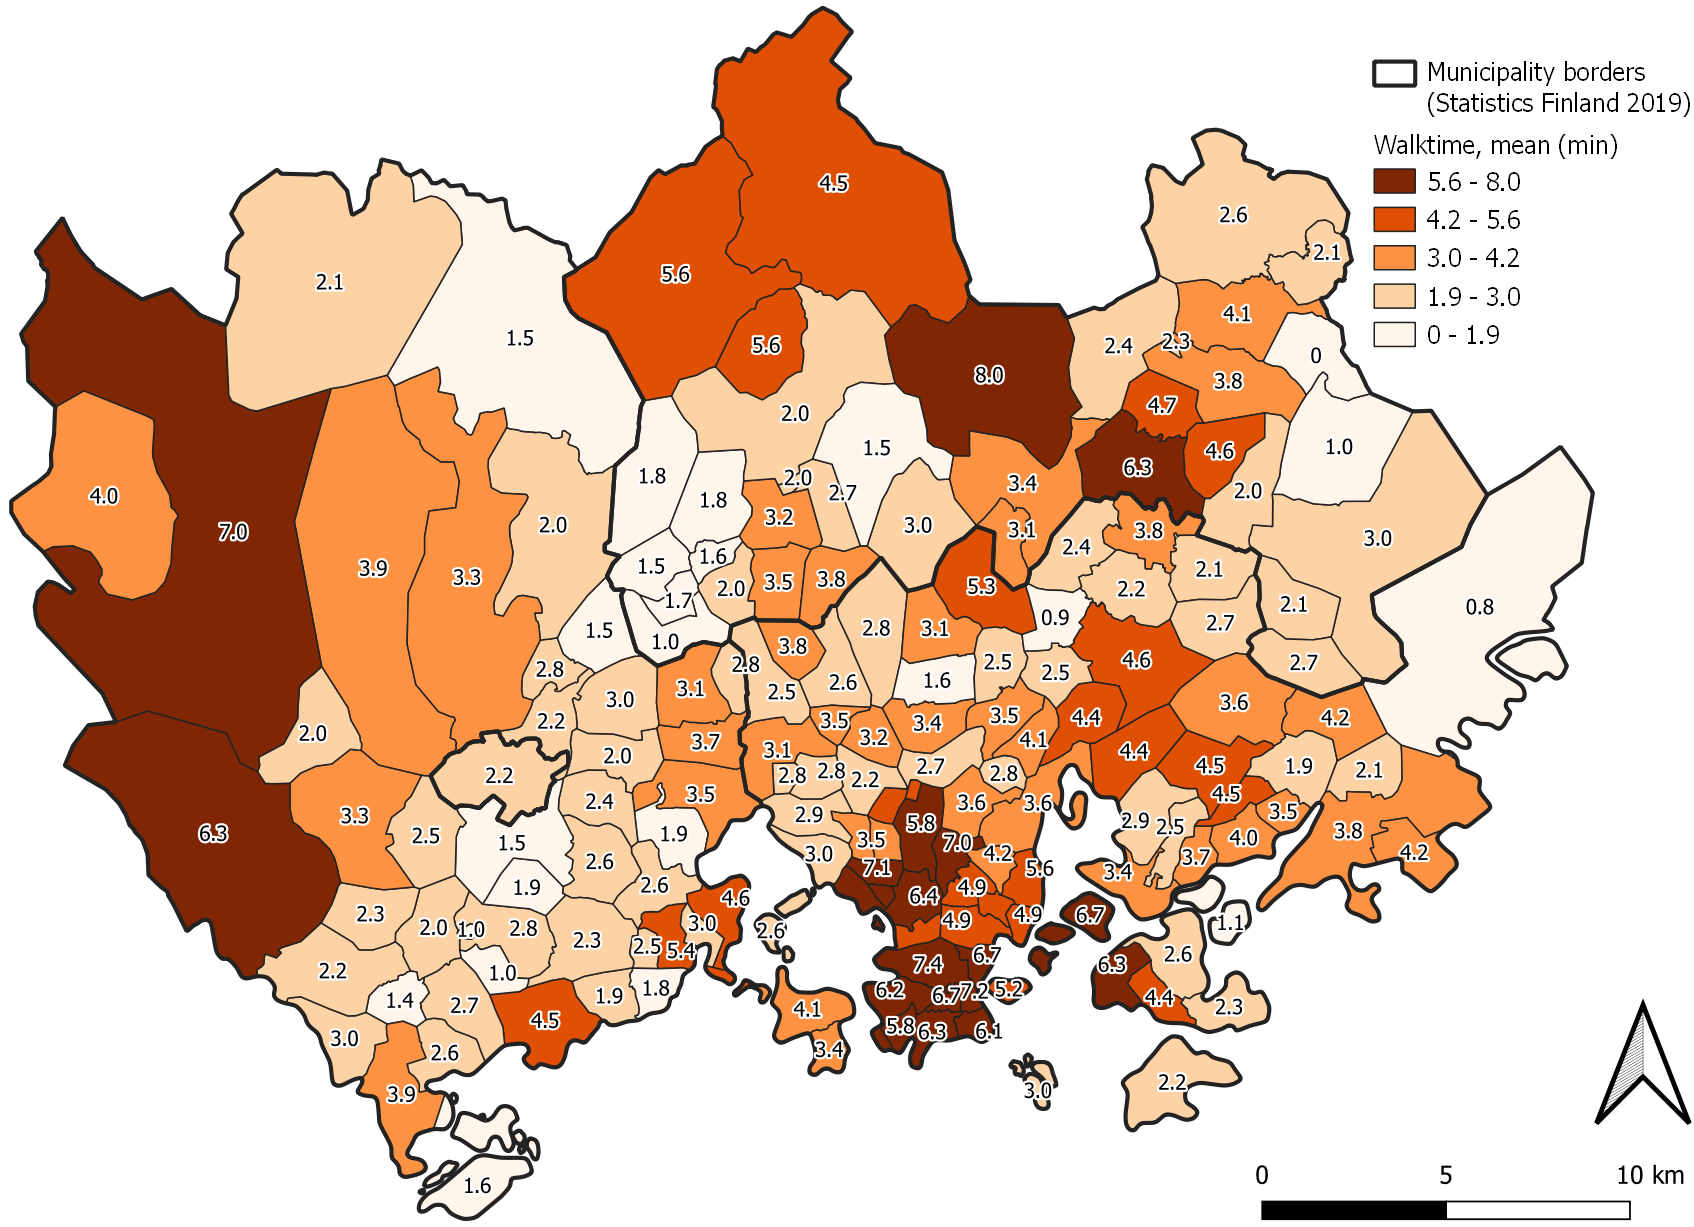
\includegraphics[width=.88\textwidth]{images/thesis_postalvis_walkmean.png}
    \caption[Walktime, mean, in the research area]{This figure illustrates the mean duration of walking from one's parked car to the final destination in each postal code area.}%
    \label{fig:postalvis_walkmean}%
\end{figure}

\begin{figure}[H]%
    \centering
    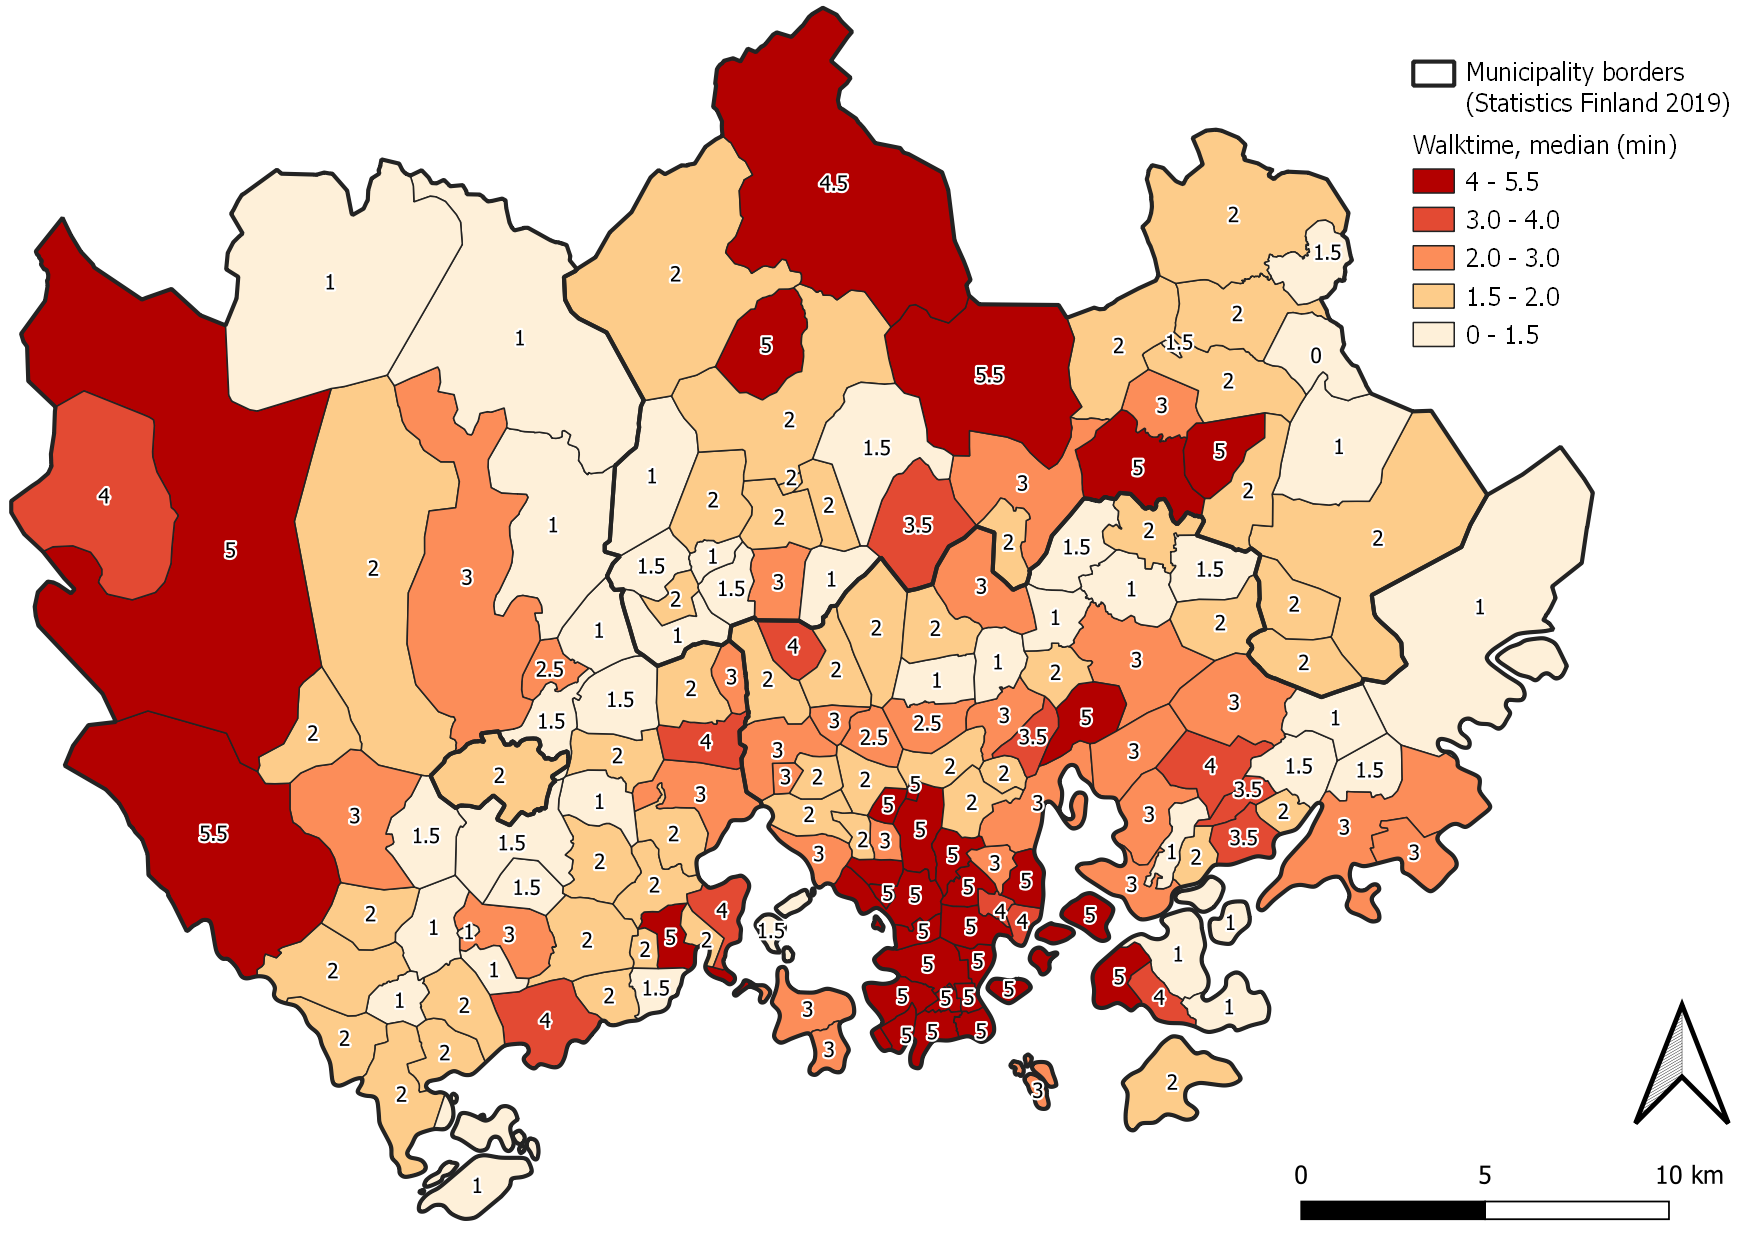
\includegraphics[width=.88\textwidth]{images/thesis_postalvis_walkmedian.png}
    \caption[Walktime, median, in the research area]{This figure illustrates the median duration of walking from one's parked car to the final destination in each postal code area.}%
    \label{fig:postalvis_walkmedian}%
\end{figure}

\newpage
\subsection{Survey findings and statistics}
\justify

The thesis survey data reveals that there are spatial differences between municipalities and regions of Helsinki Capital Region (table~\ref{tab:park_walk_subdiv}) in the durations to find a parking spot (\code{parktime}), and walking from one's parked car to the final destination (\code{walktime}). This is shown by the one-way analysis of variance test (ANOVA) that for \code{parktime} and \code{walktime} there are statistically significant differences ($p < 0.05$) between the 23 groups (municipality subdivisions, figure~\ref{fig:subdiv_placement}). In the vast majority of subdivision groups, the group sizes were sufficiently large for ANOVA analysis to be significant. An exception to this is the ANOVA test for Espoo's subdivisions using \code{parktime}. This test finishes with a less significant $p = 0.015$.

The spatial differences between subdivisions were wide-ranging, with a 5.2 minutes mean \code{parktime} in Helsinki, 3.8 minutes in Vantaa, 3.2 minutes in Espoo and lastly, 2.1 minutes in Kauniainen. Median \code{parktime} for the municipalities were 4.0, 2.0, 2.0, and 2.0 minutes, respectively. Durations to find a parking spot varied inside municipalities; in Espoo, in the subdivision of Pohjois-Espoo mean \code{parktime} was 1.7 minutes (median 1.0 minute) while the same value for Suur-Matinkylä was 4.3 minutes (3.0 min). From all the subdivisions in the research area, the subdivision representing the center of Helsinki, Helsinki Southern, had the the longest mean \code{parktime}, 7.3 minutes (5.0 min). Kauniainen ranked as fourth with a \code{parktime} values 2.1 minutes mean and 2.0 minutes median.

Viewing \code{walktime} through subdivisions, longest \code{walktime} was found from Espoo's Suur-Kauklahti (mean 6.3 min, median 5.5 min). In Helsinki, the Southern subdivision's durations were the second longest (mean 6.3 min, median 5.0 min) with Vantaa's top values reaching 5.8 minutes mean and 5.0 median in Tikkurila. Kauniainen's \code{walktime} values were more moderate with 2.2 minutes mean and 2.0 minutes median.

When comparing specific subdivisions, we can observe finer details in the survey dataset. For example, comparing \code{parktime} in Espoo's Suur-Tapiola and Vantaa's Aviapolis gives no statistical significance with ANOVA ($p = 0.12$). However, a test with Suur-Tapiola and Helsinki's Southern subdivision is statistically significant ($p < 0.05$). It is interesting, that an ANOVA \code{parktime} comparison of Espoo's Suur-Leppävaara and Helsinki's Northeastern subdivisions -- both important subcenters of their respective cities -- produces no statistical significance ($p = 0.84$). 

Differences of Espoo's Vanha-Espoo and Helsinki's Östersundom subdivisions viewed with \code{walktime} gives a faint statistical significance with ANOVA ('.', $p = 0.06$). Differences of Vanha-Espoo and Vantaa's Tikkurila proved not statistically significant (' ', $p = 0.20$). It is interesting that important city centers receive different results from the ANOVA test. For example, differences in \code{walktime} are statistically significant (’***’, $p \leq 0.001$) between Vantaa's Myyrmäki and Tikkurila subdivisions. \code{walktime} differences of Espoo's Suur-Matinkylä and Suur-Leppävaara are not (' ', $p = 0.13$). The same case stands for Helsinki's Southeastern and Western subdivisions of which differences were not identified as statistically significant (' ', $p = 0.76$). However, varying degrees of significance is found for the same subdivision comparison pairs when using \code{parktime} as the explanatory variable: Myyrmäki--Tikkurila achieves high statistical significance (’***’, $p \leq 0.001$), while Suur-Matinkylä--Suur-Leppävaara ('**', $p = 0.007$), and Southeastern--Western ('**', $p = 0.007$) get moderate significance.

% \textcolor{red}{290720 kun verrataan kahta subdiviä (2 ryhmää), käytetään anovaa ja katsotaan merkitsevyys. Suur-Tapiola ja Aviapolis oli " ", ei-merkitsevä, Suur-Tapiola ja Helsinki Southern ***. Kirjoita muutamasta parista, joissa ***. Vois mainita yhden kiinnostavan, missä parkkiaikojen ero on kohinaa (Tapiola ja Aviapolis). Muista tää sama walktimelle.} \\
% \textcolor{red}{290720 katso muut muuttujat niin, että mukana kaikki subdivit, onko merkitsevyyttä anovassa} \\
% \textcolor{red}{290720 parktime: verrataan arki-viikonloppu, **, walktime: ei ole ollenkaan!} \\
% \textcolor{red}{voi tutkii myös kaupunkien erot pareina, mutta tämä taitaa tarvita koodia} \\
% \textcolor{red}{parktime Espoossa ja Helsingissä (eri tarkastelut), espoossa ei niin väliä milloin pysäköi, kun taas helsingissä merkittävämmät erot} \\
% \textcolor{red}{raportoi nyt ne mun omatkin variaapelit!} \\
%\textcolor{red}{comparison-sovelluksen tulokset: muutama esimerkkireitti ja kerro pct:stä} \\
% 290720 vantaan timeofday arkiruuhka ja arkiei-ruuhka oudot tulokset, arkiruuhka nopeampi. Mutta tämä on ei-merkitsevä anovan mukaan! synninpäästö
% 290720 espoon timeofdayn pienet erot ovat kohinaa anovan mukaan (ei-merkitsevä), can't specify ei mukana
% 290720 anova kertoo että onks vähintään JOKU 1 ryhmä merkitsevästi eri kuin muut, sitten seuraavaksi pitäis tutkii lisää, vaikka pareittain



%https://www.researchgate.net/post/Is_there_a_minimum_number_per_group_neccessary_for_an_ANOVA
%anova - ryhmän koko anovassa
% interpret anova table in r
%http://www.understandingdata.net/2017/05/11/anova-tables-in-r/
%https://www.statisticssolutions.com/sample-size-calculation-for-one-way-anovas-in-dissertations-and-theses/

% levene näyttää vain vähän eri, niin ei oo välii, sitten pitäis kattoo keskihajontaa
%anova pitäis olla ok koska 20 tapausta jo riittävä tuloksen löytymiseen 
%voin todeta, että on tilastolliseti merkitsevä ero, sitten vaan raportoi mikä on ero, esim espoo vs helsinki
%anova todistaa, että kaikilla esim "subdiveillä" ei ole samoja arvoja
%-- parittaiset t-testit jos haluaa kahden paikan välillä testailla
%-- viikonloppuaikojen sisällä varianssi ja viikonpäivän varianssi, kuinka paljon varianssista se selittää
%-- power-analyysi?? Eta-squared (eta2)

%https://statistics.laerd.com/spss-tutorials/one-way-anova-using-spss-statistics-2.php
%LINKISTÄ: therefore, there is a statistically significant difference in the
%mean length of time to complete the spreadsheet problem between the different 
%courses taken.

\begin{hyphenrules}{nohyphenation}
    \begin{table}[H]
        \centering
        \caption[Parktime and walktime descriptive statistics with explanatory variable subdiv]{Parking times and walking times descriptive statistics displayed by municipalities and subdivisions (the explanatory variable \code{subdiv}). The unit of median, mean, and standard deviation is minutes. Significance codes: '***' $p \leq 0.001$, '**' $p \leq 0.01$, '*' $p \leq 0.05$, '.' $p \leq 0.1$, 'ns' $p \leq 1$.}
        \label{tab:park_walk_subdiv}
        \scalebox{0.66}
        % Column type C is a custom column which adds space to its position. Used to separate important features of this table. L aligns left.
        {\begin{tabular}{clLccccCcccccc}
            \toprule
		    & & &                                       \multicolumn{5}{c}{parktime} &          \multicolumn{5}{c}{walktime} \\
														\cmidrule(lr{\tbspace}){4-8}            \cmidrule(lr){9-13}
			& & n &                                     Median & Mean & Std.dev & Std.err & p-value & Median & Mean & Std.dev & Std.err & p-value \\
            
            \midrule
            \multirow{7}{*}{Espoo} & Pohjois-Espoo &    29 & 1 & 1.69 & 2.12 & 0.39 & &         1 & 1.86 & 1.55 & 0.29 & \\
            & Suur-Espoonlahti &                        99 & 2 & 2.88 & 3.27 & 0.33 & &         2 & 2.83 & 2.67 & 0.27 & \\
            & Suur-Kauklahti &                          10 & 2 & 3.50 & 3.69 & 1.17 & &         5.5 & 6.30 & 4.81 & 1.52 & \\
            & Suur-Leppävaara &                         176 & 2 & 3.12 & 2.94 & 0.22 & &        3 & 3.27 & 2.41 & 0.18 & \\
            & Suur-Matinkylä &                          95 & 3 & 4.28 & 4.05 & 0.42 & &         3 & 3.76 & 2.81 & 0.29 & \\
            & Suur-Tapiola &                            257 & 2 & 3.33 & 3.94 & 0.25 & &        2 & 3.84 & 3.41 & 0.21 & \\
            & Vanha-Espoo &                             80 & 2 & 2.81 & 4.00 & 0.45 & &         3 & 3.89 & 3.81 & 0.43 & \\
            % Use \arrayrulecolor to get a grey cmidrule, then revert \midrule color back to black
            \arrayrulecolor{black!30}\cmidrule(lr){2-13}
            & \textbf{Total} &                          746 & 2 & 3.23 & 3.63 & 0.13 & * &    2 & 3.52 & 3.09 & 0.11 & *** \\
            \arrayrulecolor{black}\midrule
            
            \multirow{8}{*}{Helsinki} & Central &       704 & 5 & 5.54 & 5.72 & 0.22 & &        5 & 4.91 & 3.92 & 0.15 & \\
            & Eastern &                                 360 & 2 & 3.61 & 3.41 & 0.18 & &        3 & 3.91 & 3.51 & 0.18 & \\
            & Northeastern &                            308 & 2 & 3.19 & 3.83 & 0.22 & &        3 & 3.63 & 3.47 & 0.20 & \\
            & Northern &                                162 & 1 & 2.38 & 2.73 & 0.21 & &        2 & 3.16 & 3.21 & 0.25 & \\
            & Southeastern &                            315 & 2 & 3.42 & 3.72 & 0.21 & &        2 & 3.70 & 3.79 & 0.21 & \\
            & Southern &	                            1310 & 5 & 7.26 & 6.47 & 0.18 & &       5 & 6.23 & 4.56 & 0.13 & \\
            & Western &                                 612 & 2 & 4.28 & 5.04 & 0.20 & &        3 & 3.63 & 3.15 & 0.13 & \\
            & Östersundom &                             6 & 0.5 & 0.67 & 0.82 & 0.33 & &        1 & 0.83 & 0.75 & 0.31 & \\
            \arrayrulecolor{black!30}\cmidrule(lr){2-13}
            & \textbf{Total} &                          3777 & 4 & 5.24 & 5.60 & 0.09 & *** &   4 & 4.78 & 4.10 & 0.07 & *** \\
            \arrayrulecolor{black}\midrule
            
            Kauniainen & Kauniainen &                   23 & 2 & 2.13 & 1.60 & 0.33 & --- &     2 & 2.22 & 1.28 & 0.27 & --- \\
            \midrule
            
            \multirow{7}{*}{Vantaa} & Aviapolis &       184 & 3 & 3.93 & 4.09 & 0.30 & &        3 & 4.51 & 4.27 & 0.31 & \\
            & Hakunila &                                44 & 1.5 & 2.41 & 2.89 & 0.44 & &       2 & 2.59 & 2.47 & 0.37 & \\
            & Kivistö &                                 48 & 1 & 4.69 & 6.37 & 0.92 & &         3 & 4.88 & 4.99 & 0.72 & \\
            & Koivukylä &                               40 & 1 & 2.80 & 3.74 & 0.59 & &         2 & 3.33 & 3.69 & 0.58 & \\
            & Korso &                                   50 & 2 & 2.92 & 4.43 & 0.63 & &         2 & 2.50 & 1.59 & 0.23 & \\
            & Myyrmäki &                                161 & 2 & 2.98 & 4.13 & 0.33 & &        2 & 2.83 & 3.08 & 0.24 & \\
            & Tikkurila &                               110 & 5 & 5.84 & 5.60 & 0.53 & &        5 & 5.85 & 5.15 & 0.49 & \\
            \arrayrulecolor{black!30}\cmidrule(lr){2-13}
            & \textbf{Total} &                          637 & 2 & 3.82 & 4.65 & 0.18 & *** &    3 & 3.98 & 4.11 & 0.16 & *** \\
            \arrayrulecolor{black}\midrule
            
            All & \textbf{Total} &                      5183 & 3 & 4.76 & 5.29 & 0.07 & *** &   3 & 4.49 & 3.99 & 0.06 & *** \\
            \bottomrule
        \end{tabular}}
    \end{table}
\end{hyphenrules}

The municipalities of Helsinki Capital Region show varying results when \code{parktime} and \code{walktime} were viewed against the thesis survey variable \code{timeofday}, the time of day for parking one's car (table~\ref{tab:park_walk_timeofday}). Highest values for each choice were found in Helsinki, where \code{parktime} mean was highest for \textit{Weekday, rush hour} (mean 5.7 min, median 5 min). Interestingly, none of the other municipalities had \textit{Weekday, rush hour} as the longest choice. In Espoo the choice \textit{Can't specify, no usual time} was the longest (mean 3.8 min, median 2.0 min), while in Vantaa the choice \textit{Weekday, other than rush hour} took the top position (mean 4.2 min, median 2.0 min). In Kauniainen survey participants reported the longest \code{parktime} values during the weekend (mean 3.0 min, median 3.0 min).

Furthermore, Helsinki also had the longest \code{walktime} values when viewed against \code{timeofday}. In the capital it took the longest to walk from one's car to the final destination on weekend (mean 5.1 min, median 5.0 min). For Espoo, survey participants again reported the highest \code{walktime} value for the choice \textit{Can't specify, no usual time} (mean 4.0 min, median 3.0 min). In Vantaa one had to walk the longest from the car to the final destination during weekday's rush hour (mean 4.7 min, median 3.0 min), while in Kauniainen weekend private car users spent the longest time walking from their car to their destination (mean 2.6 min, median 2.0 min).

The ANOVA test yielded varying results when comparing choices of \code{timeofday} inside municipalities of Helsinki Capital Region. Highly significant differences between the time of day of parking and walking from one's car to the final destination were only detected in Helsinki, where both \code{parktime} and \code{walktime} received significance code of ***. The corresponding test for Espoo produced a weaker statistical significance with \code{parktime} ('*', $p = 0.04$) and \code{walktime} ('*', $p = 0.02$). The ANOVA tests were entirely non-significant while Vantaa's ANOVA test testing \code{timeofday} produced a non-significant result for \code{parktime} and a weak significance for \code{walktime} ('.', $p = 0.07$).

Groups were excluded from the variable \code{timeofday} in a test to see if it would enhance statistical significance of differences between the rest of the groups. This proved unsuccessful. For example, statistically significant differences could not be found for \code{timeofday} groups when concentrating on Vantaa and \code{parktime}. Each group was successively excluded from the test and additionally hypothetically different times of day were compared to each other (\textit{Weekday, rush hour}--\textit{Weekend}).

\begin{hyphenrules}{nohyphenation}
    \begin{table}[H]
        \centering
        \caption[timeofday descriptives]{Parking times and walking times descriptive statistics with explanatory variable \code{timeofday}. The unit of median, mean, and standard deviation is minutes. Significance codes: '***' $p \leq 0.001$, '**' $p \leq 0.01$, '*' $p \leq 0.05$, '.' $p \leq 0.1$, 'ns' $p \leq 1$.}
        \label{tab:park_walk_timeofday}
        \scalebox{0.66}
        {\begin{tabular}{clLccccCcccccc}
            \toprule
            & & &                                           \multicolumn{5}{c}{parktime} &          \multicolumn{5}{c}{walktime} \\
                                                            \cmidrule(lr{\tbspace}){4-8}            \cmidrule(lr){9-13}
            & & n &                                         Median & Mean & Std.dev & Std.err & p-value & Median & Mean & Std.dev & Std.err & p-value \\
            
            \midrule
            \multirow{5}{*}{Espoo} & Weekday, rush hour &   174 & 2 & 3.26 & 3.91 & 0.30 & &        2 & 3.60 & 3.18 & 0.24 & \\
            & Weekday, other than rush hour &               227 & 2 & 2.79 & 3.00 & 0.20 & &        2 & 3.05 & 2.59 & 0.17 & \\
            & Weekend &                                     155 & 2 & 3.11 & 2.81 & 0.23 & &        3 & 3.57 & 2.88 & 0.23 & \\
            & Can't specify, no usual time &                190 & 2 & 3.82 & 4.48 & 0.33 & &        3 & 3.96 & 3.62 & 0.26 & \\
            \arrayrulecolor{black!30}\cmidrule(lr){2-13}
            & \textbf{Total} &                              746 & 2 & 3.23 & 3.63 & 0.13 & * &      2 & 3.52 & 3.09 & 0.11 & * \\
            \arrayrulecolor{black}\midrule
            
            \multirow{5}{*}{Helsinki} & Weekday, rush hour & 900 & 5 & 5.71 & 6.38 & 0.21 & &       5 & 4.99 & 4.29 & 0.14 & \\
            & Weekday, other than rush hour &               1360 & 4 & 5.41 & 5.42 & 0.15 & &       4 & 4.83 & 3.97 & 0.11 & \\
            & Weekend &                                     698 & 3.5 & 4.94 & 4.76 & 0.18 & &      5 & 5.06 & 4.28 & 0.16 & \\
            & Can't specify, no usual time &                819 & 3 & 4.68 & 5.58 & 0.19 & &        3 & 4.23 & 3.90 & 0.14 & \\
            \arrayrulecolor{black!30}\cmidrule(lr){2-13}
            & \textbf{Total} &                              3777 & 4 & 5.24 & 5.60 & 0.09 & *** &   4 & 4.78 & 4.10 & 0.07 & *** \\
            \arrayrulecolor{black}\midrule
            
            \multirow{5}{*}{Kauniainen} & Weekday, rush hour & 5 & 1 & 1.80 & 1.79 & 0.80 & &       2 & 2.40 & 1.67 & 0.75 & \\
            & Weekday, other than rush hour &               8 & 2 & 2.50 & 1.85 & 0.65 & &          2 & 2.38 & 1.19 & 0.42 & \\
            & Weekend &                                     5 & 3 & 3.00 & 1.22 & 0.55 & &          2 & 2.60 & 1.52 & 0.68 & \\
            & Can't specify, no usual time &                5 & 1 & 1.00 & 0.71 & 0.32 & &          1 & 1.40 & 0.55 & 0.24 & \\
            \arrayrulecolor{black!30}\cmidrule(lr){2-13}
            & \textbf{Total} &                              23 & 2 & 2.13 & 1.60 & 0.33 & $ns$ &    2 & 2.22 & 1.28 & 0.27 & $ns$ \\
            \arrayrulecolor{black}\midrule
            
            \multirow{5}{*}{Vantaa} & Weekday, rush hour &  152 & 2 & 3.84 & 4.95 & 0.40 & &        3 & 4.71 & 5.32 & 0.43 & \\
            & Weekday, other than rush hour &               188 & 2 & 4.25 & 5.39 & 0.39 & &        3 & 3.75 & 3.41 & 0.25 & \\
            & Weekend &                                     141 & 2 & 3.65 & 3.44 & 0.29 & &        3 & 3.97 & 3.94 & 0.33 & \\
            & Can't specify, no usual time &                156 & 2 & 3.45 & 4.32 & 0.35 & &        2 & 3.54 & 3.58 & 0.29 & \\
            \arrayrulecolor{black!30}\cmidrule(lr){2-13}
            & \textbf{Total} &                              637 & 2 & 3.82 & 4.65 & 0.18 & $ns$ &   3 & 3.98 & 4.11 & 0.16 & . \\
            \arrayrulecolor{black}\midrule
            
            All & \textbf{Total} &                          5183 & 3 & 4.76 & 5.29 & 0.07 & *** &   3 & 4.49 & 3.99 & 0.06 & *** \\
            \bottomrule
        \end{tabular}}
    \end{table}
\end{hyphenrules}

The thesis survey data showed marked differences between parking place types in the research area (table~\ref{tab:park_walk_parkspot}). Viewing \code{parktime} and \code{walktime} through \code{parkspot} reveals that in all research area municipalities, excluding Kauniainen, parking on the side of the street took the most time. In Helsinki, street parking parking took a mean 6.3 minutes (5.0 min median) while in Vantaa the corresponding value was 5.8 minutes (4.0 min median). In Espoo street parking was slightly shorter with a mean of 4.1 minutes (3.0 min median). In Kauniainen, street parking took a mean duration of 2.33 minutes (1.0 min median), with parking in a parking lot narrowly surpassing street parking with a mean 2.35 minutes (2.0 min median). In all research area municipalities parking in parking garages took more time than parking on parking lots. For Helsinki, these values were overall highest with a small margin, 4.0 minutes to 3.9 minutes mean (3.0--2.0 min median) for \textit{Parking garage} and \textit{Parking lot}, respectively. Corresponding values in Vantaa were 4.0-3.5 minutes mean (3.0--2.0 min median) and in Espoo 3.6 minutes compared to 2.9 minutes mean (3.0--2.0 min median). In Kauniainen no parking garage responses were recorded, with the value \textit{Parking lot} receiving a mean duration of 2.3 minutes (2.0 min median).

Walking to one's destination from the parked car also was the longest when participants had parked on the side of the street, again excepting Kauniainen. \code{walktime} was highest in Vantaa, with a mean duration of 5.15 minutes (5.0 min median). Helsinki's values came in second at 5.12 minutes mean (5.0 min median). Espoo and Kauniainen's figures were at 4.0 and 2.3 minutes mean, respectively. As with \code{parktime}, the hierarchy of values being greater after parking in a parking garage rather than parking lot was also demonstrated in \code{walktime}. The longest durations were recorded in Helsinki with 5.0 to 4.3 minutes mean (5.0--3.0 min median) for \textit{Parking garage} and \textit{Parking lot}, respectively. In Vantaa the values were 4.8--3.6 minutes mean (4.0--2.0 min median) and in Espoo 3.9--3.3 minutes mean (3.0--2.0 min median). 

The thesis survey data shows that \code{parktime} and \code{walktime} in private parking lots or non-personal reserved parking spots was under two minutes mean ($\leq$ 1.0 min median) in all municipalities, with the exception of Vantaa's \code{walktime}, where the group \textit{Private or reserved} received a mean duration of 2.2 minutes.

The ANOVA test for the explanatory variable \code{parkspot} and response variables \code{parktime} and \code{walktime} showed strong statistical significance for differences between parking spot types and study area municipalities. However, while the three largest research area municipalities had this state ('***' for Helsinki, Espoo, and Vantaa), Kauniainen received non-significant results from the ANOVA test for both \code{parktime} and \code{walktime}. In the cases of all research area municipalities, a better significance for differences between \code{parkspot} groups could be attained by excluding the group \textit{Other}, if only slightly. When testing with a more limited set of \textit{parkspot} groups, such as only testing differences of \textit{Parking lot} and \textit{Parking garage}, all statistical significance would be lost with the exception of Espoo, where statistical significance for the differences would position at '*', $p = 0.02$. All municipalities except Kauniainen would also receive substantial statistical significance when testing for differences between the group \textit{On the side of street} and \textit{Private or reserved} ('***', $p \leq 0.001$).

\begin{hyphenrules}{nohyphenation}
    \begin{table}[H]
        \centering
        \caption[parkspot descriptives]{Parking times and walking times descriptive statistics with explanatory variable \code{parkspot}. The unit of median, mean, and standard deviation is minutes. Significance codes: '***' $p \leq 0.001$, '**' $p \leq 0.01$, '*' $p \leq 0.05$, '.' $p \leq 0.1$, 'ns' $p \leq 1$.}
        \label{tab:park_walk_parkspot}
        \scalebox{0.66}
        {\begin{tabular}{clLccccCcccccc}
            \toprule
			& & &                                           \multicolumn{5}{c}{parktime} &          \multicolumn{5}{c}{walktime} \\
															\cmidrule(lr{\tbspace}){4-8}            \cmidrule(lr){9-13}
			& & n &                                         Median & Mean & Std.dev & Std.err & p-value & Median & Mean & Std.dev & Std.err & p-value \\
            
            \midrule
            \multirow{6}{*}{Espoo} & On the side of street & 150 & 3 & 4.15 & 3.91 & 0.32 & &       3 & 3.97 & 3.01 & 0.25 & \\
            & Parking lot &                                 363 & 2 & 2.91 & 3.66 & 0.19 & &        2 & 3.33 & 3.28 & 0.17 & \\
            & Parking garage &                              171 & 3 & 3.64 & 2.90 & 0.22 & &        3 & 3.95 & 2.53 & 0.19 & \\
            & Private or reserved &                         49 & 1 & 1.12 & 1.24 & 0.18 & &         1 & 1.88 & 1.82 & 0.26 & \\
            & Other &                                       13 & 2 & 4.08 & 7.89 & 2.19 & &         2 & 4.23 & 5.66 & 1.57 & \\
            \arrayrulecolor{black!30}\cmidrule(lr){2-13}
            & \textbf{Total} &                              746 & 2 & 3.23 & 3.63 & 0.13 & *** &    2 & 3.52 & 3.09 & 0.11 & *** \\
            \arrayrulecolor{black}\midrule
            
            \multirow{6}{*}{Helsinki} & On the side of street & 2241 & 5 & 6.35 & 6.08 & 0.13 & &   5 & 5.12 & 4.06 & 0.09 & \\
            & Parking lot &                                 817 & 2 & 3.91 & 4.78 & 0.17 & &        3 & 4.35 & 4.34 & 0.15 & \\
            & Parking garage &                              522 & 3 & 4.01 & 3.85 & 0.17 & &        5 & 5.01 & 3.94 & 0.17 & \\
            & Private or reserved &                         178 & 1 & 1.19 & 2.12 & 0.16 & &        1 & 1.98 & 2.39 & 0.18 & \\
            & Other &                                       19 & 2 & 3.00 & 3.51 & 0.81 & &         1 & 2.95 & 3.41 & 0.78 & \\
            \arrayrulecolor{black!30}\cmidrule(lr){2-13}
            & \textbf{Total} &                              3777 & 4 & 5.24 & 5.60 & 0.09 & *** &   4 & 4.78 & 4.10 & 0.07 & *** \\
            \arrayrulecolor{black}\midrule
            
            \multirow{6}{*}{Kauniainen} & On the side of street & 3 & 1 & 2.33 & 2.31 & 1.33 & &    1 & 2.33 & 2.31 & 1.33 & \\
            & Parking lot &                                 17 & 2 & 2.35 & 1.54 & 0.37 & &         2 & 2.41 & 1.12 & 0.27 & \\
            & Parking garage &                              --- & --- & --- & --- & --- & &         --- & --- & --- & --- & \\
            & Private or reserved &                         2 & 0.5 & 0.50 & 0.71 & 0.50 & &        1 & 1.00 & 0.00 & 0.00 & \\
            & Other &                                       1 & 1 & 1.00 & --- & --- & &            1 & 1.00 & --- & --- & \\
            \arrayrulecolor{black!30}\cmidrule(lr){2-13}
            & \textbf{Total} &                              23 & 2 & 2.13 & 1.60 & 0.33 & $ns$ &    2 & 2.22 & 1.28 & 0.27 & $ns$ \\
            \arrayrulecolor{black}\midrule
            
            \multirow{6}{*}{Vantaa} & On the side of street & 108 & 4 & 5.81 & 6.09 & 0.59 & &      4.5 & 5.15 & 4.98 & 0.48 & \\
            & Parking lot &                                 341 & 2 & 3.51 & 4.25 & 0.23 & &        2 & 3.62 & 3.76 & 0.20 & \\
            & Parking garage &                              127 & 3 & 4.06 & 4.33 & 0.38 & &        4 & 4.81 & 4.32 & 0.38 & \\
            & Private or reserved &                         55 & 1 & 1.49 & 2.76 & 0.37 & &         1 & 2.18 & 2.58 & 0.35 & \\
            & Other &                                       6 & 1 & 2.50 & 3.83 & 1.57 & &          1 & 2.17 & 3.87 & 1.58 & \\
            \arrayrulecolor{black!30}\cmidrule(lr){2-13}
            & \textbf{Total} &                              637 & 2 & 3.82 & 4.65 & 0.18 & *** &    3 & 3.98 & 4.11 & 0.16 & *** \\
            \arrayrulecolor{black}\midrule
            
            All & \textbf{Total} &                          5183 & 3 & 4.76 & 5.29 & 0.07 & *** &   3 & 4.49 & 3.99 & 0.06 & *** \\
            \bottomrule
        \end{tabular}}
    \end{table}
\end{hyphenrules}

A view to the thesis survey data variables \code{parktime} and \code{walktime} through explanatory variable \code{likert} point out that area familiarity does not translate into efficient parking or short walks from one's car to the final destination of one's journey (table~\ref{tab:park_walk_likert}).

The statistical significance of differences between groups for the explanatory variable \code{likert} were varying. On the other hand, Helsinki and Espoo got a $p$ value under $0.01$, while the identical test for Vantaa and Kauniainen resulted in non-significant conclusion.

\begin{hyphenrules}{nohyphenation}
    \begin{table}[H]
        \centering
        \caption[likert descriptives]{Parking times and walking times descriptive statistics with explanatory variable \code{likert}. The unit of median, mean, and standard deviation is minutes. Significance codes: '***' $p \leq 0.001$, '**' $p \leq 0.01$, '*' $p \leq 0.05$, '.' $p \leq 0.1$, 'ns' $p \leq 1$.}
        \label{tab:park_walk_likert}
        \scalebox{0.66}
        {\begin{tabular}{clLccccCcccccc}
            \toprule
			& & &                                           \multicolumn{5}{c}{parktime} &          \multicolumn{5}{c}{walktime} \\
															\cmidrule(lr{\tbspace}){4-8}            \cmidrule(lr){9-13}
			& & n &                                         Median & Mean & Std.dev & Std.err & p-value & Median & Mean & Std.dev & Std.err & p-value \\
            
            \midrule
            \multirow{6}{*}{Espoo} & Extremely familiar &   306 & 1 & 2.66 & 3.30 & 0.19 & &        2 & 3.12 & 3.07 & 0.18 & \\
            & Moderately familiar &                         224 & 3 & 3.68 & 3.51 & 0.23 & &        3 & 3.75 & 2.87 & 0.19 & \\
            & Somewhat familiar &                           130 & 2 & 3.35 & 3.52 & 0.31 & &        3 & 3.64 & 2.70 & 0.24 & \\
            & Slightly familiar &                           74 & 2 & 4.08 & 5.08 & 0.59 & &         3 & 4.39 & 4.20 & 0.49 & \\
            & Not at all familiar &                         12 & 2.5 & 2.67 & 1.61 & 0.47 & &       2 & 2.67 & 1.97 & 0.57 & \\
            \arrayrulecolor{black!30}\cmidrule(lr){2-13}
            & \textbf{Total} &                              746 & 2 & 3.23 & 3.63 & 0.13 & ** &     2 & 3.52 & 3.09 & 0.11 & ** \\
            \arrayrulecolor{black}\midrule
            
            \multirow{6}{*}{Helsinki} & Extremely familiar & 1695 & 3 & 4.84 & 5.63 & 0.14 & &      3 & 4.17 & 3.85 & 0.09 & \\
            & Moderately familiar &                         1172 & 5 & 5.94 & 6.09 & 0.18 & &       5 & 5.35 & 4.26 & 0.12 & \\
            & Somewhat familiar &                           572 & 4 & 5.07 & 4.58 & 0.19 & &        5 & 5.06 & 3.77 &0.16 & \\
            & Slightly familiar &                           282 & 4 & 5.24 & 4.98 & 0.30 & &        5 & 5.59 & 4.99 & 0.30 & \\
            & Not at all familiar &                         56 & 2.5 & 4.12 & 4.96 & 0.66 & &       3.5 & 4.59 & 3.62 & 0.48 & \\
            \arrayrulecolor{black!30}\cmidrule(lr){2-13}
            & \textbf{Total} &                              3777 & 4 & 5.24 & 5.60 & 0.09 & *** &   4 & 4.78 & 4.10 & 0.07 & *** \\
            \arrayrulecolor{black}\midrule
            
            \multirow{6}{*}{Kauniainen} & Extremely familiar & 14 & 1 & 1.79 & 1.58 & 0.42 & &      2 & 2.21 & 1.37 & 0.37 & \\
            & Moderately familiar &                         2 & 3.5 & 3.50 & 3.54 & 2.50 & &        3 & 3.00 & 2.83 & 2.00 & \\
            & Somewhat familiar &                           4 & 2 & 1.75 & 0.50 & 0.25 & &          2 & 1.75 & 0.50 & 0.25 & \\
            & Slightly familiar &                           2 & 3.5 & 3.50 & 0.71 & 0.50 & &        2.5 & 2.50 & 0.71 & 0.50 & \\
            & Not at all familiar &                         1 & 3 & 3.00 & --- & --- & &            2 & 2.00 & --- & --- & \\
            \arrayrulecolor{black!30}\cmidrule(lr){2-13}
            & \textbf{Total} &                              23 & 2 & 2.13 & 1.60 & 0.33 & $ns$ &    2 & 2.22 & 1.28 & 0.27 & $ns$ \\
            \arrayrulecolor{black}\midrule
            
            \multirow{6}{*}{Vantaa} & Extremely familiar &  267 & 1 & 3.51 & 4.93 & 0.30 & &        2 & 3.68 & 4.05 & 0.25 & \\
            & Moderately familiar &                         198 & 3 & 4.19 & 4.28 & 0.30 & &        3 & 4.34 & 4.12 & 0.29 & \\
            & Somewhat familiar &                           99 & 2 & 4.10 & 4.79 & 0.48 & &         3 & 4.48 & 4.73 & 0.48 & \\
            & Slightly familiar &                           59 & 2 & 3.92 & 4.74 & 0.62 & &         2 & 3.64 & 3.47 & 0.45 & \\
            & Not at all familiar &                         14 & 2 & 2.21 & 1.42 & 0.38 & &         2 & 2.29 & 1.38 & 0.37 & \\
            \arrayrulecolor{black!30}\cmidrule(lr){2-13}
            & \textbf{Total} &                              637 & 2 & 3.82 & 4.65 & 0.18 & $ns$ &   3 & 3.98 & 4.11 & 0.16 & $ns$ \\
            \arrayrulecolor{black}\midrule
            
            All & \textbf{Total} &                          5183 & 3 & 4.76 & 5.29 & 0.07 & *** &   3 & 4.49 & 3.99 & 0.06 & *** \\
            \bottomrule
        \end{tabular}}
    \end{table}
\end{hyphenrules}

\begin{hyphenrules}{nohyphenation}
    \begin{table}[H]
        \centering
        \caption[articifial descriptives]{Parking times and walking times descriptive statistics with explanatory variable \code{articifial}. The unit of median, mean, and standard deviation is minutes. Significance codes: '***' $p \leq 0.001$, '**' $p \leq 0.01$, '*' $p \leq 0.05$, '.' $p \leq 0.1$, 'ns' $p \leq 1$.}
        \label{tab:park_walk_artificial}
        \scalebox{0.66}
        {\begin{tabular}{clLccccCcccccc}
            \toprule
			& & &                                           \multicolumn{5}{c}{parktime} &          \multicolumn{5}{c}{walktime} \\
															\cmidrule(lr{\tbspace}){4-8}            \cmidrule(lr){9-13}
			& & n &                                         Median & Mean & Std.dev & Std.err & p-value & Median & Mean & Std.dev & Std.err & p-value \\
            
            \midrule
            \multirow{6}{*}{Espoo} & Fully built &          319 & 2 & 3.69 & 4.08 & 0.23 & &        3 & 3.96 & 3.35 & 0.19 & \\
            & Predominantly built &                         204 & 2 & 3.35 & 3.19 & 0.22 & &        3 & 3.24 & 2.36 & 0.17 & \\
            & Moderately built &                            59 & 1 & 2.22 & 2.68 & 0.35 & &         2 & 2.88 & 2.94 & 0.38 & \\
            & Some built &                                  76 & 1.5 & 2.63 & 2.97 & 0.34 & &       2 & 2.53 & 1.85 & 0.21 & \\
            & Scarcely built &                              88 & 1 & 2.45 & 3.64 & 0.39 & &         3 & 3.89 & 4.08 & 0.44 & \\
            \arrayrulecolor{black!30}\cmidrule(lr){2-13}
            & \textbf{Total} &                              746 & 2 & 3.23 & 3.63 & 0.13 & ** &     2 & 3.52 & 3.09 & 0.11 & *** \\
            \arrayrulecolor{black}\midrule
            
            \multirow{6}{*}{Helsinki} & Fully built &       2476 & 4 & 5.34 & 5.79 & 0.12 & &       4 & 4.87 & 4.11 & 0.08 & \\
            & Predominantly built &                         590 & 5 & 6.06 & 5.53 & 0.23 & &        5 & 5.06 & 4.00 & 0.16 & \\
            & Moderately built &                            468 & 3 & 4.43 & 4.90 & 0.23 & &        3 & 4.05 & 3.68 & 0.17 & \\
            & Some built &                                  182 & 2 & 4.01 & 4.68 & 0.35 & &        3 & 4.85 & 4.96 & 0.37 & \\
            & Scarcely built &                              61 & 2 & 2.92 & 3.83 & 0.49 & &         3 & 3.90 & 4.21 & 0.54 & \\
            \arrayrulecolor{black!30}\cmidrule(lr){2-13}
            & \textbf{Total} &                              3777 & 4 & 5.24 & 5.60 & 0.09 & *** &   4 & 4.78 & 4.10 & 0.07 & *** \\
            \arrayrulecolor{black}\midrule
            
            \multirow{6}{*}{Kauniainen} & Fully built &     23 & 2 & 2.13 & 1.60 & 0.33 & &         2 & 2.22 & 1.28 & 0.27 & \\
            & Predominantly built &                         --- & --- & --- & --- & --- & &         --- & --- & --- & --- & \\
            & Moderately built &                            --- & --- & --- & --- & --- & &         --- & --- & --- & --- & \\
            & Some built &                                  --- & --- & --- & --- & --- & &         --- & --- & --- & --- & \\
            & Scarcely built &                              --- & --- & --- & --- & --- & &         --- & --- & --- & --- & \\
            \arrayrulecolor{black!30}\cmidrule(lr){2-13}
            & \textbf{Total} &                              23 & 2 & 2.13 & 1.60 & 0.33 & --- &     2 & 2.22 & 1.28 & 0.27 & --- \\
            \arrayrulecolor{black}\midrule
            
            \multirow{6}{*}{Vantaa} & Fully built &         109 & 5 & 5.68 & 5.49 & 0.53 & &        5 & 5.56 & 5.27 & 0.50 & \\
            & Predominantly built &                         257 & 2 & 3.75 & 4.10 & 0.26 & &        3 & 4.18 & 3.92 & 0.24 & \\
            & Moderately built &                            27 & 1 & 2.30 & 3.31 & 0.64 & &         2 & 2.44 & 1.85 & 0.36 & \\
            & Some built &                                  179 & 2 & 3.47 & 4.95 & 0.37 & &        2 & 3.42 & 3.82 & 0.29 & \\
            & Scarcely built &                              65 & 1 & 2.57 & 3.92 & 0.49 & &         2 & 2.69 & 3.05 & 0.38 & \\
            \arrayrulecolor{black!30}\cmidrule(lr){2-13}
            & \textbf{Total} &                              637 & 2 & 3.82 & 4.65 & 0.18 & *** &    3 & 3.98 & 4.11 & 0.16 & *** \\
            \arrayrulecolor{black}\midrule
            
            All & \textbf{Total} &                          5183 & 3 & 4.76 & 5.29 & 0.07 & *** &   3 & 4.49 & 3.99 & 0.06 & *** \\
            \bottomrule
        \end{tabular}}
    \end{table}
\end{hyphenrules}

\begin{hyphenrules}{nohyphenation}
    \begin{table}[H]
        \centering
        \caption[ykr\_zones descriptives]{Parking times and walking times descriptive statistics with explanatory variable \code{ykr\_zone}. The unit of median, mean, and standard deviation is minutes. Significance codes: '***' $p \leq 0.001$, '**' $p \leq 0.01$, '*' $p \leq 0.05$, '.' $p \leq 0.1$, 'ns' $p \leq 1$.}
        \label{tab:park_walk_ykrzone}
        \scalebox{0.6}
        {\begin{tabular}{clLccccCcccccc}
            \toprule
        	& & &                                           \multicolumn{5}{c}{parktime} &              \multicolumn{5}{c}{walktime} \\
        													\cmidrule(lr{\tbspace}){4-8}                \cmidrule(lr){9-13}
        	& & n &                                         Median & Mean & Std.dev & Std.err & p-value & Median & Mean & Std.dev & Std.err & p-value \\
            
            \midrule
            \multirow{8}{*}{Espoo} & Keskustan jalankulkuvyöhyke &  --- & --- & --- & --- & --- & &     --- & --- & --- & --- & \\
            & Keskustan reunavyöhyke &                              --- & --- & --- & --- & --- & &     --- & --- & --- & --- & \\
            & Alakeskuksen jalankulkuvyöhyke &                      211 & 3 & 3.78 & 3.62 & 0.25 & &    3 & 4.12 & 2.98 & 0.20 & \\
            & Intensiivinen joukkoliikennevyöhyke &                 278 & 2 & 3.72 & 4.05 & 0.24 & &    3 & 3.58 & 3.02 & 0.18 & \\
            & Joukkoliikennevyöhyke &                               57 & 1 & 2.07 & 2.01 & 0.27 & &     2 & 2.07 & 1.57 & 0.21 & \\
            & Autovyöhyke &                                         99 & 1 & 1.93 & 2.23 & 0.22 & &     2 & 2.59 & 2.86 & 0.29 & \\
            & novalue &                                             101 & 2 & 2.65 & 3.71 & 0.37 & &    3 & 3.85 & 3.85 & 0.38 & \\
            \arrayrulecolor{black!30}\cmidrule(lr){2-13}
            & \textbf{Total} &                                      746 & 2 & 3.23 & 3.63 & 0.13 & *** & 2 & 3.52 & 3.09 & 0.11 & *** \\
            \arrayrulecolor{black}\midrule
            
            \multirow{8}{*}{Helsinki} & Keskustan jalankulkuvyöhyke & 1157 & 5 & 7.60 & 6.42 & 0.19	& & 5 & 6.36 & 4.42 & 0.13 & \\
            & Keskustan reunavyöhyke &                              1240 & 4 & 5.39 & 5.69 & 0.16 & &   4 & 4.88 & 4.14 & 0.12 & \\
            & Alakeskuksen jalankulkuvyöhyke &                      286 & 3 & 3.92 & 3.36 & 0.20 & &    3 & 4.10 & 3.25 & 0.19 & \\
            & Intensiivinen joukkoliikennevyöhyke &                 761 & 2 & 3.07 & 3.68 & 0.13 & &    2 & 3.22 & 3.19 & 0.12 & \\
            & Joukkoliikennevyöhyke &                               167 & 1 & 2.23 & 3.53 & 0.27 & &    2 & 2.72 & 2.84 & 0.22 & \\
            & Autovyöhyke &                                         18 & 1 & 1.56 & 1.54 & 0.36 & &     1 & 2.28 & 2.30 & 0.54 & \\
            & novalue &                                             148 & 2 & 3.01 & 3.57 & 0.29 & &    3 & 3.61 & 3.31 & 0.27 & \\
            \arrayrulecolor{black!30}\cmidrule(lr){2-13}
            & \textbf{Total} &                                      3777 & 4 & 5.24 & 5.60 & 0.09 & *** & 4 & 4.78 & 4.10 & 0.07 & *** \\
            \arrayrulecolor{black}\midrule
            
            \multirow{8}{*}{Kauniainen} & Keskustan jalankulkuvyöhyke & --- & --- & --- & --- & --- & & --- & --- & --- & --- & \\
            & Keskustan reunavyöhyke &                              --- & --- & --- & --- & --- & &     --- & --- & --- & --- & \\
            & Alakeskuksen jalankulkuvyöhyke &                      --- & --- & --- & --- & --- & &     --- & --- & --- & --- & \\
            & Intensiivinen joukkoliikennevyöhyke &                 --- & --- & --- & --- & --- & &     --- & --- & --- & --- & \\
            & Joukkoliikennevyöhyke &                               23 & 2 & 2.13 & 1.60 & 0.33 & &     2 & 2.22 & 1.28 & 0.27 & \\
            & Autovyöhyke &                                         --- & --- & --- & --- & --- & &     --- & --- & --- & --- & \\
            & novalue &                                             --- & --- & --- & --- & --- & &     --- & --- & --- & --- & \\
            \arrayrulecolor{black!30}\cmidrule(lr){2-13}
            & \textbf{Total} &                                      23 & 2 & 2.13 & 1.60 & 0.33	& --- & 2 & 2.22 & 1.28 & 0.27 & --- \\
            \arrayrulecolor{black}\midrule
            
            \multirow{8}{*}{Vantaa} & Keskustan jalankulkuvyöhyke & --- & --- & --- & --- & --- & &     --- & --- & --- & --- & \\
            & Keskustan reunavyöhyke &                              --- & --- & --- & --- & --- & &     --- & --- & --- & --- & \\
            & Alakeskuksen jalankulkuvyöhyke &                      260 & 3 & 4.46 & 4.72 & 0.29 & &    3 & 4.34 & 3.91 & 0.24 & \\
            & Intensiivinen joukkoliikennevyöhyke &                 88 & 2 & 4.23 & 5.38 & 0.57 & &     2 & 4.26 & 5.00 & 0.53 & \\
            & Joukkoliikennevyöhyke &                               68 & 2 & 3.21 & 4.58 & 0.55 & &     2 & 2.78 & 2.70 & 0.33 & \\
            & Autovyöhyke &                                         98 & 1 & 2.43 & 3.62 & 0.37 & &     2 & 2.42 & 2.43 & 0.25 & \\
            & novalue &                                             123 & 2 & 3.64 & 4.49 & 0.40 & &    3 & 4.91 & 4.99 & 0.45 & \\
            \arrayrulecolor{black!30}\cmidrule(lr){2-13}
            & \textbf{Total} &                                      637 & 2 & 3.82 & 4.65 & 0.18 & ** & 3 & 3.98 & 4.11 & 0.16 & *** \\
            \arrayrulecolor{black}\midrule
            
            All & \textbf{Total} &                                  5183 & 3 & 4.76 & 5.29 & 0.07 & *** & 3 & 4.49 & 3.99 & 0.06 & *** \\
            \bottomrule
        \end{tabular}}
    \end{table}
\end{hyphenrules}

\newpage
\subsection{Travel time comparison application findings}
\justify

moi